\documentclass{article}
\usepackage{enumitem} 
\usepackage{mathtools}% http://ctan.org/pkg/mathtools
\usepackage[makeroom]{cancel}
\usepackage{amsmath,amsfonts,amsthm,amssymb,amsopn,bm}
\usepackage[margin=.9in]{geometry}
\usepackage{graphicx}
\usepackage{url}
\usepackage[usenames,dvipsnames]{color}
\usepackage{fancyhdr}
\usepackage{multirow}
\newcommand{\field}[1]{\mathbb{#1}}
\newcommand{\1}{\mathbf{1}}
\newcommand{\E}{\mathbb{E}} 
\renewcommand{\P}{\mathbb{P}}
\newcommand{\R}{\field{R}} % real domain
% \newcommand{\C}{\field{C}} % complex domain
\newcommand{\F}{\field{F}} % functional domain

\newcommand{\T}{^{\textrm T}} % transpose

\def\diag{\text{diag}}

%% operator in linear algebra, functional analysis
\newcommand{\inner}[2]{#1\cdot #2}
\newcommand{\norm}[1]{\left\|#1\right\|}
\newcommand{\twonorm}[1]{\|#1\|_2^2}
% operator in functios, maps such as M: domain1 --> domain 2
\newcommand{\Map}[1]{\mathcal{#1}}
\renewcommand{\theenumi}{\alph{enumi}} 

\newcommand{\Perp}{\perp \! \! \! \perp}

\newcommand\independent{\protect\mathpalette{\protect\independenT}{\perp}}
\def\independenT#1#2{\mathrel{\rlap{$#1#2$}\mkern2mu{#1#2}}}
\newcommand{\vct}[1]{\boldsymbol{#1}} % vector
\newcommand{\mat}[1]{\boldsymbol{#1}} % matrix
\newcommand{\cst}[1]{\mathsf{#1}} % constant
\newcommand{\ProbOpr}[1]{\mathbb{#1}}
\newcommand{\points}[1]{\small\textcolor{magenta}{\emph{[#1 points]}} \normalsize}
\date{{}}

%\setlength\parindent{0px}

\begin{document}
\title{Homework \#0}
\author{\normalsize{Mudi Qin}\\
\normalsize{Spring 2020, CSE 446/546: Machine Learning}\\
\normalsize{Prof. Kevin Jamieson and Prof. Jamie Morgenstern} \\
\normalsize{Due: 4/8/19  11:59 PM}\\
\normalsize{A: 37 points. B: 3 points}}
\maketitle


\section*{Probability and Statistics}
A.1 \points{2} (Bayes Rule, from Murphy exercise 2.4.) After your yearly checkup, the doctor has bad news and good news. The bad news is that you tested positive for a serious disease, and that the test is 99\% accurate (i.e., the probability of testing positive given that you have the disease is 0.99, as is the probability of testing negative given that you dont have the disease). The good news is that this is a rare disease, striking only one in 10,000 people. What are the chances that you actually have the disease? (Show your calculations as well as giving the final result.)\\

\noindent\fbox{%
    \parbox{\textwidth}{%
\begin{proof}
                
        Define event $A=\text{actually have the disease}$, event $B=$test positive. Then $\neg A=$not have the disease, $\neg B=$ test negative.\\
        In the problem, the following are given: \\
        1.$P(B|A)=P(\neg B|\neg A) = 0.99$\\
        2.$P(A)=\frac{1}{10000}$\\
        by Bayes Rule:  $P(A|B)=\frac{P(A)P(B|A)}{P(B)}= \frac{P(A)P(B|A)}{P(B|A)P(A)+P(B|\neg A)P(\neg A)}=\frac{0.0001*0.99}{0.99*0.0001+0.01*(1-.0001)}=.009803$
\end{proof}
}
}\\

A.2 For any two random variables $X,Y$ the \emph{covariance} is
  defined as
  $\text{Cov}(X,Y)=\E[(X-\E[X])(Y-\E[Y])]$. You may assume $X$ and $Y$
  take on a discrete values if you find that is easier to work with.
\begin{enumerate}
\item \points{1} If $\E[Y|X=x] = x$ show that $\text{Cov}(X,Y) = \E[(X-\E[X])^2]$.  
\item \points{1} If $X,Y$ are independent show that $\text{Cov}(X,Y)=0$.
\end{enumerate}

\noindent\fbox{%
 \parbox{\textwidth}{%
\begin{proof}
        (a) With the given information, it can be proven that $E[X]=E[Y]$ for any given $x:$\\
        \begin{align*}
                E[Y|X=x] = \sum_{y \in Y} y P(Y=y|X=x) &= x \\
                \sum_{y \in Y} y \frac{P(Y=y,X=x)}{P(X=x)}&= x \\
                \sum_{y \in Y} y P(Y=y,X=x)&= x P(X=x)\\
        \end{align*}
                I noticed the Expected value of X can be calculated from the LHS\\
        \begin{align*}
                \sum_{x \in X}\sum_{y \in Y} y P(Y=y,X=x)&= \sum_{x \in X} x P(X=x)\\
                \sum_{y \in Y} y\underbrace{\sum_{x \in X}P(Y=y,X=x)}_{\text{sum marginal probability across x}}&= \sum_{x \in X} x P(X=x)\\
                \sum_{y \in Y} y P(Y=y)&= \sum_{x \in X} x P(X=x)\\
                E[X] &= E[Y]
        \end{align*}

With the bellow two formula: \\
\begin{enumerate}[label=(\roman*)]
        \item law of expectation: $E[Y]=E_z[Y|Z]$ 
        \item $E(g(X)h(Y)|X) = g(x)E(h(Y)|X)$
\end{enumerate}

        Rewrtie the formula for $Cov(X,Y)$:\\ 
        \[
        \begin{aligned}
                Cov(X,Y)&= E[(X-E[X])(Y-E[Y])]\\
                        &=E_X[E[(X-E[X])(Y-E[Y])]|X]\\
                        &\stackrel{\text{by (ii)}}{=} E_X[(X-E[X])E[(Y-\underbrace{E(X)}_{\text{as proven}})|X]]\\
                        &= E_X[(X-E[X])(X-E[X])]\\
                        &= E[(X-E[X])^2]\\
        \end{aligned}
\]
\end{proof}
}
}

\noindent\fbox{%
    \parbox{\textwidth}{%
\begin{proof}
        (b)\\
        
        \begin{align*}
                Cov(X,Y)&= E[(X-E[X])(Y-E[Y])]\\
                 &= E[(XY -XE[Y] - YE[X]+E[X]E[Y])]\\
                 &=\underbrace{E[XY]}_{\text{X,Yindependent}}-E[XE[Y]] -E[YE[X]]+E[X]E[Y]\\
                 &=E[X]E[Y]-E[X]E[Y]-E[X]E[Y]+E[X]E[Y]\\
                 &=0
        \end{align*}
\end{proof}
}
}
A.3 Let $X$ and $Y$ be independent random variables with PDFs given by $f$ and $g$, respectively. Let $h$ be the PDF of the random variable $Z = X+Y$.
\begin{enumerate}
	\item \points{2} Show that $h(z) = \int_{-\infty}^\infty f(x) g( z - x ) d x $.  (If you are more comfortable with discrete probabilities, you can instead derive an analogous expression for the discrete case,  and then you should give a one sentence explanation as to why your expression is analogous to the continuous case.).
	\item \points{1} If $X$ and $Y$ are both independent and uniformly distributed on $[0,1]$ (i.e. $f(x)=g(x)=1$ for $x \in [0,1]$ and $0$ otherwise) what is $h$, the PDF of $Z=X+Y$?
\end{enumerate}

\noindent\fbox{%
    \parbox{\textwidth}{%
\begin{proof}
        (a)\\
        Define the marginal distribution $p(x,y)=P(X=x,Y=y)$. Define the CDF $H(z)=P(X+Y \leq z)$ \\
        $$H(z)=P(X+Y\leq z)= \int_{x \in R} \int_{-\infty}^{z-x} p(x,y)dydx$$
        from $H(z)$, we can get $h(z)$:
        \[
\begin{aligned}
        h(z)&=\frac{d}{dz}H(z) \\
            &=\frac{d}{dz}\int_{x \in R} \int_{-\infty}^{z-x} p(x,y)dydx \\
            &=\int_{x \in R} \underbrace{\frac{d}{dz}\int_{-\infty}^{z-x} p(x,y)dy}_{\text{Fundamental thereom of calculus}}dx \\
            &=\int_{x \in R} \underbrace{p(x,z-x)}_{independence}dx \\
            &=\int_{x \in R} f(x)g(z-x)dx
\end{aligned}
\]
\end{proof}
}}



\noindent\fbox{%
    \parbox{\textwidth}{%

\begin{proof}
        (b)\\
        $Y,X ~ U(0,1)$ where the PDF follows: 
        \[ f(x)=
                \begin{cases}
1,   \qquad 0 \leq x \leq 1 \\
                       0,  \qquad otherwise 
                \end{cases}
                \]
                The PDF for Z=X+Y could be found by:\\
                \[ h(z)=\int_{x \in R} f(x)f(z-x)=f(x)*f(x)=
                \begin{cases}
x,  \qquad 0 \leq x < 1 \\
2-x, \qquad 1 \leq x \leq 2\\ 
                       0,  \qquad otherwise 
                \end{cases}
                \]
\end{proof}
}}\\

A.4 \points{1} A random variable $X \sim \mathcal{N}(\mu, \sigma^2)$ is Gaussian distributed with mean $\mu$ and variance $\sigma^2$. Given that for any $a,b \in \R$, we have that $Y = aX + b$ is also Gaussian, find $a,b$ such that $Y \sim \mathcal{N}(0,1)$.\\


\noindent\fbox{%
    \parbox{\textwidth}{%
\begin{proof}
        \[
\begin{aligned}
        E[X]&=\mu\\
        E[aX+b]&=a\mu+b
\end{aligned}
        \]
for continuous variable the variance can be calculated as :\\
        \[
\begin{aligned}
        Var(X)&=\int_{x \in \mathcal{R}}(x-\mu)^{2} f(x)dx =\sigma^2\\         Var(aX+b)&=\int_{x \in \mathcal{R}}((ax+b)-(a\mu+b))^{2} f(x)dx \\ 
              &= a^2\int_{x \in \mathcal{R}}(x-\mu)^{2} f(x)dx \\ 
              &= a^2 \sigma ^2
\end{aligned}
        \]
        Given that $\mu=0$, $\sigma^2 = 1$, $a,b$ can be solved as follow:\\
        \[
\begin{cases}
                a\mu+b=0\\
                a^2 \sigma^2=1
\end{cases}
 \implies a =\pm\frac{1}{\sigma}, b= \mp \frac{\mu}{\sigma}  
        \]
\end{proof}
}}\\

A.5 \points{2} For a random variable $Z$, its mean and variance are defined as $\E[Z]$ and $\E[(Z-\E[Z])^2]$, respectively.
Let $X_1,\dots,X_n$ be independent and identically distributed random variables, each with mean $\mu$ and variance $\sigma^2$. 
If we define $\widehat{\mu}_n = \frac{1}{n} \sum_{i=1}^n X_i$, what is the mean and variance of $\sqrt{n}(\widehat{\mu}_n - \mu)$?\\

\noindent\fbox{%
    \parbox{\textwidth}{%
\begin{proof}
        Define $Z=\sqrt{n}(\widehat{\mu}_n - \mu)$,
        then expectation $E[Z]$ and Variance $Var[Z]$ can be calculated as follow:\\ 
        \[
        \begin{aligned}
                E[Z]&=E[\sqrt{n}(\widehat{\mu}_n-\mu)]\\
                    &= \sqrt{n}E[\frac{1}{n}\sum_{i=1}^{n}X_i-\mu]\\ 
                    &= \sqrt{n}(\frac{1}{n}\sum_{i=1}^{n}E[X_i]-E[\mu])\\ 
                    &=0
        \end{aligned}
\]
        \[
        \begin{aligned}
                Var[Z]&=E[(Z-E[Z])^2]\\
                      &=E[Z^2]-\cancelto{0}{E[2ZE[Z]]}+\cancelto{0}{E[(E[Z])^2]}\\
                      &=E[\sqrt{n}(\widehat{\mu}_n-\mu)^2]\\
                      &=nE[(\widehat{\mu}_n-\mu)^2]\\
                      &=nE[\widehat{\mu}_n^2-2\widehat{\mu}_n \mu + \mu^2]\\
                      &=nE[\widehat{\mu}_n^2]-nE[2\widehat{\mu}_n \mu] + nE[\mu^2]\\
                      &=nE[\widehat{\mu}_n^2]\underbrace{-n2\mu E[\widehat{\mu}_n] + n\mu^2}_{=-n\mu^2}\\
        \end{aligned}
\]
In the above equation, $E[\widehat{\mu}_n^2]$ remains unknown.Start with the variance of $\widehat{\mu}_n$.
\[
        \begin{aligned}
                Var[\widehat{\mu}_n] &= Var[\frac{1}{n} \sum_{i=1}^{n}X_i] = \frac{1}{n^2}(Var[X_1]+Var[X_2]+...+Var[X_n]) = \frac{1}{n^2} n\sigma^2 = \frac{\sigma^2}{n}\\
                Var[\widehat{\mu}_n] &= E[\widehat{\mu}_n^2]-(E[\widehat{\mu}])^2 = E[\widehat{\mu}_n^2]-\mu^2\\
                E[\widehat{\mu}_n^2]&=\mu^2+\frac{\sigma^2}{n}
        \end{aligned}
        \]
        Plug this back to get: $$Var[Z] =Var[\sqrt{n}(\widehat{\mu}_n - \mu)]= n(\mu^2+\frac{\sigma^2}{n})-n\mu^2 = \sigma^2$$


\end{proof}
}}\\

A.6 If $f(x)$ is a PDF, the cumulative distribution function (CDF)
  is  defined as $F(x) = \int_{-\infty}^x f(y) dy$.  For any function
  $g : \R \rightarrow \R$ and random variable $X$ with PDF $f(x)$,
  recall that the expected value of $g(X)$ is defined as
  $\E[g(X)] = \int_{-\infty}^\infty g(y) f(y) dy$. For a boolean event
  $A$, define $\1\{ A \}$ as $1$ if $A$ is true, and $0$
  otherwise. Thus, $\1\{ x \leq a \}$ is $1$ whenever $x \leq a$ and
  $0$ whenever $x > a$.  Note that $F(x) = \E[\1\{X \leq x\}]$.  Let
  $X_1,\dots,X_n$ be \emph{independent and identically distributed}
  random variables with CDF $F(x)$.  Define
  $\widehat{F}_n(x) = \frac{1}{n} \sum_{i=1}^n \1\{X_i \leq
  x\}$. Note, for every $x$,
  that $\widehat{F}_n(x)$ is an \emph{empirical estimate} of  $F(x)$.
  You may use your answers to the previous problem.
  \begin{enumerate}
  \item \points{1} For any $x$, what is $\E[ \widehat{F}_n(x) ]$?
  \item \points{1} For any $x$, the variance of $\widehat{F}_n(x)$ is $\E[ ( \widehat{F}_n(x) -
    F(x) )^2 ]$.  Show that $\textrm{Variance}(\widehat{F}_n(x)) = \frac{F(x)(1-F(x))}{n}$. \\
%    (Hint: Consider what independence implies.)
  \item \points{1} Using your answer to b, show that
    for all $x\in \R$, we have  $\displaystyle \E[ ( \widehat{F}_n(x) - F(x) )^2 ] \leq \tfrac{1}{4n}$.  
  \end{enumerate} 


\noindent\fbox{%
    \parbox{\textwidth}{%
  \begin{proof}
          (a).\\
          $$E[\widehat{F}_n(x)]=E[\frac{1}{n}\sum_{i=1}\1\{X_i \leq x\}] =\frac{1}{n}\sum_{i=1}^{n}E[\1\{X_i \leq x\}]=F(x)$$
  \end{proof}
  }}\\


\noindent\fbox{%
    \parbox{\textwidth}{%
  \begin{proof}
          (b).\\
          Noticed that by independence of $X_i$, Variance of sum $=$ Sum of Variance. 
          $$Var[\widehat{F}_n(x)]=Var[\frac{1}{n}\sum_{i=1}\1\{X_i \leq x\}]=\frac{1}{n^2}\sum_{i=1}^{n}Var[\1\{X_i\leq x\}]$$
          realizing that $X_i$ follows Bernouli ditribution: $X_i \sim Ber(p)$. Variance of each single event is $Var = F(x)(1-F(x))$. Hence, the variance can be simplified like the following:\\

          $$Var[\widehat{F}_n(x)]=\frac{1}{n^2}\sum_{i=1}^{n}Var[\1\{X_i\leq x\}]=\frac{1}{n^2}(nF(x)(1-F(x)))=\frac{F(x)(1-F(x))}{n}$$
  \end{proof}
  }}\\


\noindent\fbox{%
    \parbox{\textwidth}{%
  \begin{proof}
          (c).\\
          As can be observed, PDF $F(x) \in [0,1]$. 
          $$F_{max}(x) =  \operatorname*{argman}_{F(x)} F(x)(1-F(x))=\frac{1}{2} \implies Max(F(x)(1-F(x)))=\frac{1}{2}*\frac{1}{2}=\frac{1}{4}$$
          Therefore, $$Var[\widehat{F}_n(x)]\leq \frac{1}{4}*\frac{1}{n}$$
  \end{proof}
  }
  }\\

B.1  \points{1} Let $X_1,\dots,X_n$ be $n$ independent and identically distributed random variables drawn unfiromly at random from $[0,1]$. If $Y = \max\{X_1,\dots,X_n\}$ then find $\E[Y]$.\\

\noindent\fbox{%
    \parbox{\textwidth}{%
\begin{proof}
        Known that the distribtion of $X_i \sim U(0,1)$. Then the CDF: $$F(X_i\leq x)= \begin{cases}
                x, \qquad x \in [0,1]\\
0, \qquad otherwise
        \end{cases}$$
        The CDF of all values among i.i.d. $X_i$ is less than or equal to x is H(x):
        $$H(x)=P(Y \leq x)=P(X_1\leq x, X_2 \leq x,...,X_n\leq x) =F(x_1)F(x_2)...F(x_n) = x^n$$
     To get PDF from CDF: 
     $$\frac{d}{dx}H(x)=nx^{n-1}$$
     The expected value: 
     $$E[Y]=\int_{x \in R} xnx^{n-1}dx = \frac{n}{n+1}$$
        
\end{proof}
}
}\\

\section*{Linear Algebra and Vector Calculus}
A.7 (Rank) Let $A = \begin{bmatrix} 1 & 2 & 1 \\ 1 & 0 & 3 \\ 1 & 1 & 2 \end{bmatrix}$ and $B = \begin{bmatrix} 1 & 2 & 3 \\ 1 & 0 & 1 \\ 1 & 1 & 2 \end{bmatrix}$.
For each matrix $A$ and $B$,
\begin{enumerate} 
	\item \points{2} what is its rank? 
	\item \points{2} what is a (minimal size) basis for its column span?
\end{enumerate}

\noindent\fbox{%
    \parbox{\textwidth}{%
\begin{proof}
        (a).\\
     After row reduction, rank(A)=2 and rank(B)=2.
\end{proof}
    }}\\

\noindent\fbox{%
    \parbox{\textwidth}{%
\begin{proof}
        (b).\\
        For A, the first two columns are pivoting columns. For B, the first 2 columns are the pivoting columns. The two matrices share the same set of minimum spanning set\\
        $$span(A)= \begin{pmatrix*}
\begin{pmatrix*}
                1\\1\\1
\end{pmatrix*}
\begin{pmatrix*}
                2\\0\\1
\end{pmatrix*}
                
        \end{pmatrix*} $$
\end{proof}
    }}\\
A.8 (Linear equations) Let $A = \begin{bmatrix} 0 & 2 & 4 \\ 2 & 4 & 2 \\ 3 & 3 & 1 \end{bmatrix}$, $b = \begin{bmatrix} -2 & -2 & -4 \end{bmatrix}^T$, and $c=\begin{bmatrix} 1 & 1 & 1 \end{bmatrix}^T$.
\begin{enumerate}
	\item \points{1} What is $Ac$?
	\item \points{2} What is the solution to the linear system $Ax = b$? (Show your work).
\end{enumerate}

\noindent\fbox{%
    \parbox{\textwidth}{%
\begin{proof}
        (a).\\
        \[
        \begin{pmatrix*}
                0&2&4\\2&4&2\\3&3&1
        \end{pmatrix*}
        \begin{pmatrix*}
                        1\\1\\1
                \end{pmatrix*}
                =
                \begin{pmatrix*}
                                6\\8\\7
                \end{pmatrix*}
        \]
\end{proof}
}}\\

\noindent\fbox{%
    \parbox{\textwidth}{%
\begin{proof}
        (b).\\
        \[
        \begin{pmatrix*}
                0&2&4\\2&4&2\\3&3&1
        \end{pmatrix*}
        \begin{pmatrix*}
                        x_1\\x_2\\x_3
                \end{pmatrix*}
                =
                \begin{pmatrix*}
                                -2\\-2\\-4
                \end{pmatrix*} 
        \]\\
switch row1 and row3:\\
\[
\begin{pmatrix*}
        3&3&1\\
        2&4&2\\
        0&2&4
\end{pmatrix*}
\begin{pmatrix*}
                x_1\\x_2\\x_3
        \end{pmatrix*}
        =
        \begin{pmatrix*}
                        -4\\-2\\-2
        \end{pmatrix*}
\]\\
$r2*\frac{3}{2}-r1$ :\\
\[
\begin{pmatrix*}
        3&3&1\\
        3&6&3\\
        0&2&4
\end{pmatrix*}
\begin{pmatrix*}
                x_1\\x_2\\x_3
        \end{pmatrix*}
        =
        \begin{pmatrix*}
                        -4\\-3\\-2
        \end{pmatrix*}
\]\\
$r3*\frac{3}{2}-r2$
\[
\begin{pmatrix*}
        3&3&1\\
        3&6&3\\
        0&0&3
\end{pmatrix*}
\begin{pmatrix*}
                x_1\\x_2\\x_3
        \end{pmatrix*}
        =
        \begin{pmatrix*}
                        -4\\1\\-3
        \end{pmatrix*}
\]\\
$$\mathbf{x}=\begin{pmatrix}
        -2\\
        1\\
        -1\\
\end{pmatrix}$$
\end{proof}
}}\\

A.9 (Hyperplanes) Assume $w$ is an $n$-dimensional vector and $b$ is a scalar. A hyperplane in $\R^n$ is the set $\{x : x\in \R^n,\text{ s.t. } w^T x + b = 0\}$.
\begin{enumerate}
	\item \points{1} ($n=2$ example) Draw the hyperplane for $w=[-1,2]^T$, $b=2$? Label your axes.
	\item \points{1} ($n=3$ example) Draw the hyperplane for $w=[1,1,1]^T$, $b=0$? Label your axes.
	\item \points{2} Given some $x_0 \in \R^n$, find the \emph{squared distance} to the hyperplane defined by $w^T x + b=0$.
	In other words, solve the following optimization problem:
	\begin{align*}
	\min_x& \|x_0 - x \|^2\\
	\text{s.t. }&w^Tx +b = 0
	\end{align*}
	(Hint: if $\widetilde{x}_0$ is the minimizer of the above problem, note that $\| x_0 - \widetilde{x}_0 \| = | \frac{w^T(x_0 - \widetilde{x}_0)}{\|w\|} |$. What is $w^T \widetilde{x}_0$?)
\end{enumerate} 

\noindent\fbox{%
    \parbox{\textwidth}{%
\begin{proof}
        (a).\\
        $\mathbf{x} \in R^{2}$, $\mathbf{x}=[x_1,x_2]^{T}$, then $<w,x>+b = w_1 x_1 + w_2 x_2 +b = -1x_1 + 2x_2+2$. This is a line as plotted below:\\
(b).\\
        $\mathbf{x} \in R^{3}$, $\mathbf{x}=[x_1,x_2,x_3]^{T}$, then $<w,x>+b = w_1 x_2 + w_2 x_2 + w_3 x_2 +b=x_1+x_2+x_3$. This is a line as plotted below:\\
\begin{center}
        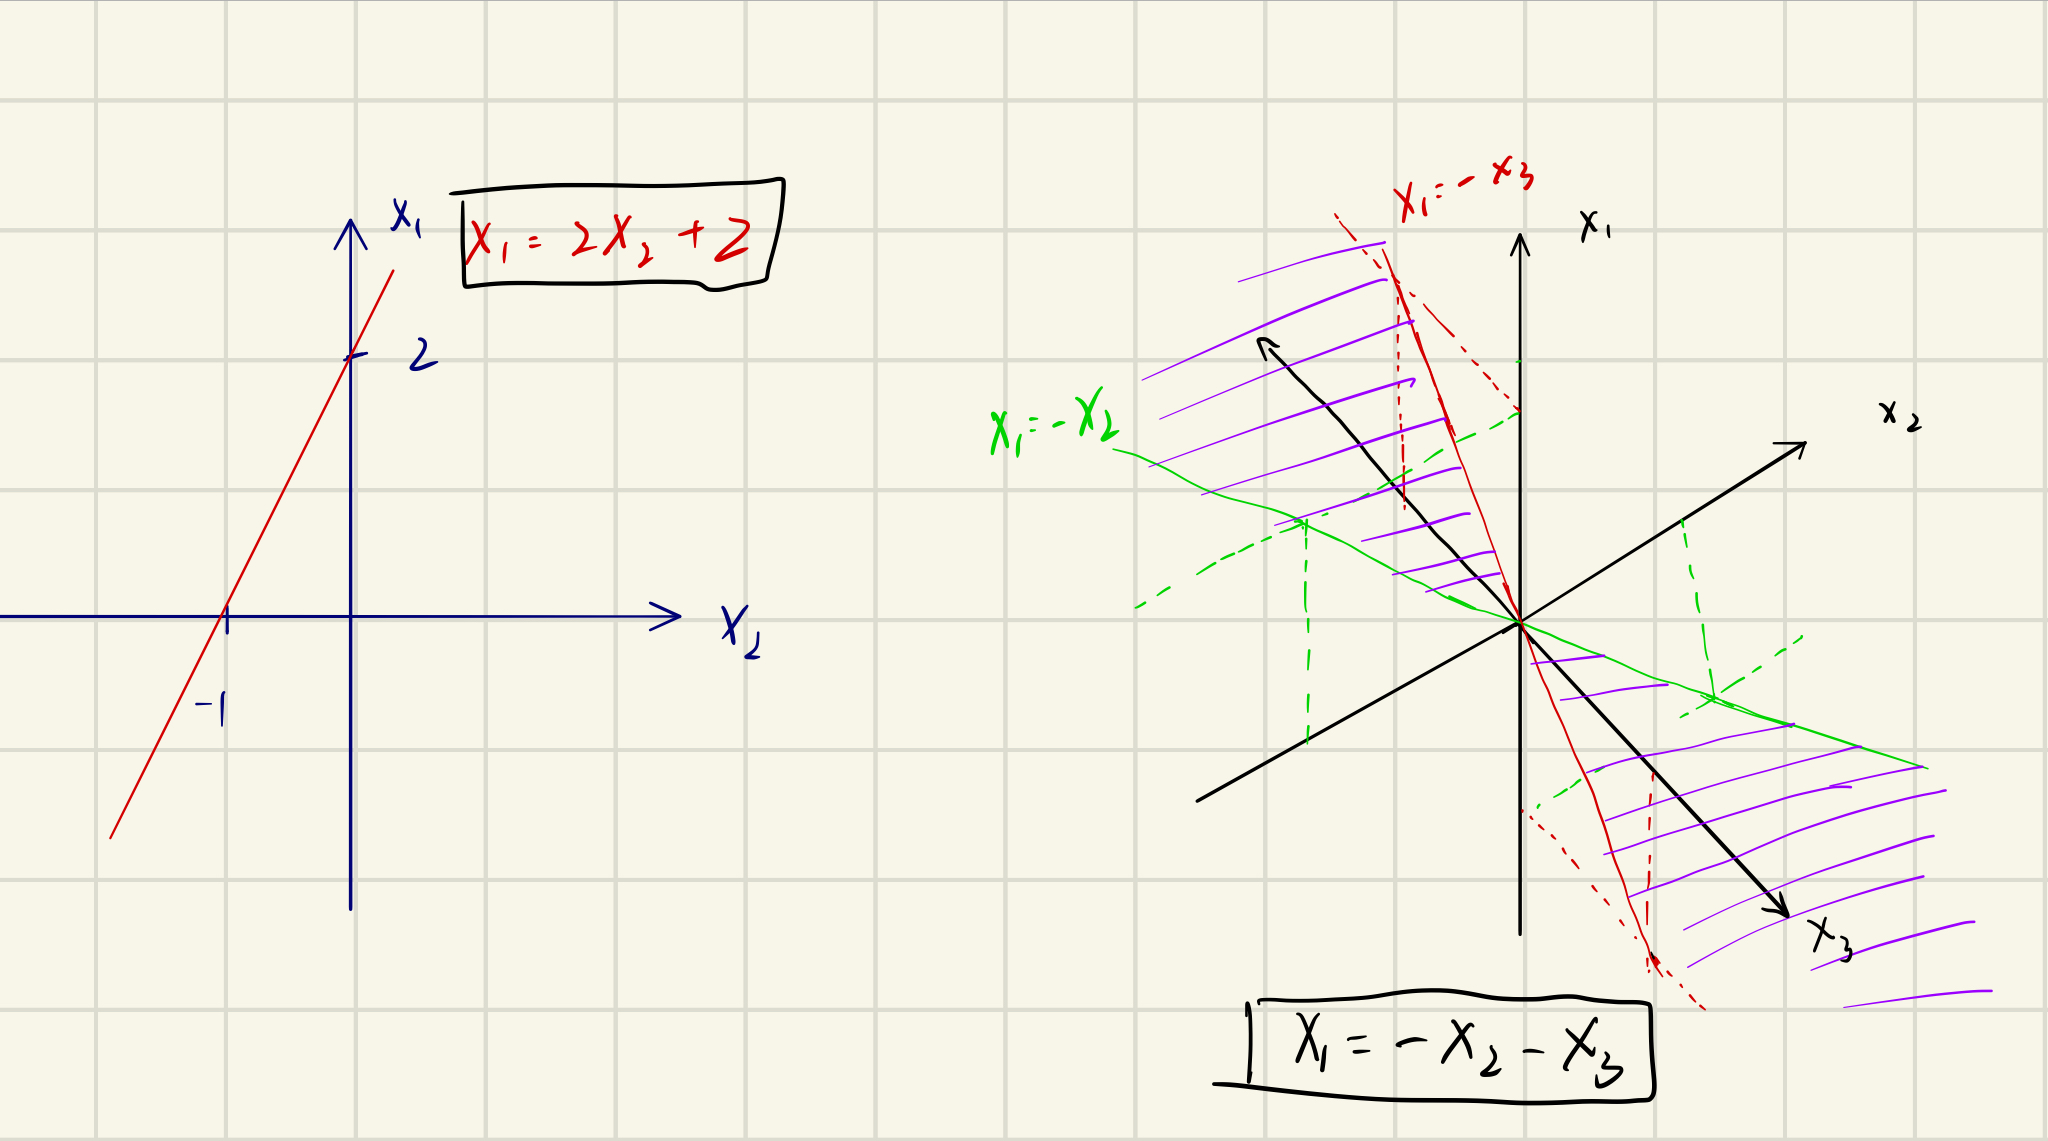
\includegraphics[height=5cm, width=15cm]{56655.jpg}
\end{center}
\end{proof}
}}\\

\noindent\fbox{%
\parbox{\textwidth}{%
\begin{proof}
        The equation of the surface is $\mathbf{w}^{T}\mathbf{x}+b=0$. The norm of the plane is $$\mathbf{n}=\frac{\mathbf{w}^{T}}{||\mathbf{w^T}||}$$
        the distance of any given point $\mathbf{x_0}$ in the $\mathbb{R}^n$ to the surface/hyperplane is given by:$$d=|<\mathbf{n},\mathbf{v}>|$$
        where $\mathbf{v}$ is calculated as $\mathbf{v}=\mathbf{x_0}-\widetilde{\mathbf{x}_0}$, $\widetilde{\mathbf{x}_0}$ is the projection of $x_0$ onto the surface. Because $\widetilde{\mathbf{x}_0}$ is on the surface, it satisfies $\mathbf{w}^{T} \widetilde{\mathbf{x}_0}+b=0. b=- \mathbf{w}^{T} \widetilde{\mathbf{x}_0}$, Therefore: \\
$$d= \| x_0 - \widetilde{x}_0 \| = | \frac{w^T(x_0 - \widetilde{x}_0)}{\|w\|} |= | \frac{w^Tx_0 +b)}{\|w\|} |$$

\end{proof}
}}\\

A.10 For possibly non-symmetric $\mat{A}, \mat{B} \in \R^{n \times n}$ and $c \in \R$, let $f(x, y) = x^T \mat{A} x + y^T \mat{B} x + c$. Define $\nabla_z f(x,y) = \begin{bmatrix} \frac{\partial f(x,y)}{\partial z_1} & \frac{\partial f(x,y)}{\partial z_2} & \dots & \frac{\partial f(x,y)}{\partial z_n} \end{bmatrix}^T$.  
\begin{enumerate}
	\item \points{2} Explicitly write out the function $f(x, y)$ in terms of the components $A_{i,j}$ and $B_{i,j}$ using appropriate summations over the indices.
	\item \points{2} What is $\nabla_x f(x,y)$ in terms of the summations over indices \emph{and} vector notation?
	\item \points{2} What is $\nabla_y f(x,y)$ in terms of the summations over indices \emph{and} vector notation?
\end{enumerate}

\noindent\fbox{%
\parbox{\textwidth}{%
\begin{proof}
        (a).\\
        Start off by computing $\mathbf{A}\mathbf{x}$ and $\mathbf{B}\mathbf{x}:$ 
        $$\mathbf{A}\mathbf{x}=\begin{bmatrix} 
                \sum_{j=1}^{n} A_{1j}x_{j}\\
                \sum_{j=1}^{n} A_{2j}x_{j}\\
                \vdots\\
                \sum_{j=1}^{n} A_{nj}x_{j}\\
        \end{bmatrix}
        ,
        \mathbf{B}\mathbf{x}=\begin{bmatrix} 
                \sum_{j=1}^{n} B_{1j}x_{j}\\
                \sum_{j=1}^{n} B_{2j}x_{j}\\
                \vdots\\
                \sum_{j=1}^{n} B_{nj}x_{j}\\
        \end{bmatrix}$$
        then, $$\mathbf{x^TAx} = [x_1,x_2,x_3....,x_n] \begin{bmatrix} 
                \sum_{j=1}^{n} A_{1j}x_{j}\\
                \sum_{j=1}^{n} A_{2j}x_{j}\\
                \vdots\\
                \sum_{j=1}^{n} A_{nj}x_{j}\\
        \end{bmatrix} = \sum_{i=1}^{n}\sum_{j=1}^{n} A_{i,j}x_ix_j$$
$$\mathbf{y^TBx} = [y_1,y_2,y_3....,y_n] \begin{bmatrix} 
                \sum_{j=1}^{n} B_{1j}x_{j}\\
                \sum_{j=1}^{n} B_{2j}x_{j}\\
                \vdots\\
                \sum_{j=1}^{n} B_{nj}x_{j}\\
        \end{bmatrix} = \sum_{i=1}^{n}\sum_{j=1}^{n} B_{j,i}y_jx_i
        $$
        $$f_{x,y}= \sum_{i=1}^{n}\sum_{j=1}^{n} A_{i,j}x_ix_j + \sum_{i=1}^{n}\sum_{j=1}^{n} B_{j,i}y_jx_i+c$$
\end{proof}
}}\\

\noindent\fbox{%
\parbox{\textwidth}{%
\begin{proof}
        (b).\\
                $$\frac{d}{dx}(\mathbf{x^TAx}) = \frac{d}{dx}( \sum_{i=1}^{n}\sum_{j=1}^{n} A_{i,j}x_ix_j) = \begin{bmatrix}
                        \frac{d}{dx_1}( \sum_{i=1}^{n}\sum_{j=1}^{n} A_{i,j}x_ix_j)\\

                        \frac{d}{dx_2}( \sum_{i=1}^{n}\sum_{j=1}^{n} A_{i,j}x_ix_j) \\
                        \frac{d}{dx_3}( \sum_{i=1}^{n}\sum_{j=1}^{n} A_{i,j}x_ix_j) \\
                        \vdots\\
                        \frac{d}{dx_n}( \sum_{i=1}^{n}\sum_{j=1}^{n} A_{i,j}x_ix_j) 
                \end{bmatrix}$$
                for each entries, the calculation follows:\\
                        $$\frac{d}{dx_k}( \sum_{i=1}^{n}\sum_{j=1}^{n} A_{i,j}x_ix_j)=\frac{d}{dx_k}( \sum_{j=1}^{n} A_{k,j}x_kx_j) + \frac{d}{dx_k}( \sum_{i=1}^{n} A_{i,k}x_kx_i)=\sum_{j=1}^{n} A_{k,j}x_j +  \sum_{i=1}^{n} A_{i,k}x_i = (\mathbf{Ax})_k + (\mathbf{A^Tx})_k$$
\noindent\text{Therefore, the partial dirivative of the matrix form  $\mathbf{x^TAx}$ is: }\\
                        $$\frac{d}{dx}(\mathbf{x^TAx})=\mathbf{(A+A^{T})x}$$
Then I would want to work on the next term:\\ 
$$\mathbf{y^TBx} = \sum_{i=1}^{n}\sum_{j=1}^{n} B_{j,i}y_jx_i$$
\[
\begin{aligned}           
        \frac{d}{dx}\mathbf{y^TBx} &= \frac{d}{dx}\sum_{i=1}^{n}\sum_{j=1}^{n} B_{i,j}y_jx_i=\begin{bmatrix} 
                \sum_{j=1}^{n} B_{j,1} y_j\\ 
                \sum_{j=1}^{n} B_{j,2} y_j\\ 
                \sum_{j=1}^{n} B_{j,3} y_j\\ 
                \vdots\\
                \sum_{j=1}^{n} B_{j,n} y_j\\ 
        \end{bmatrix} = \mathbf{y^TB}
\end{aligned}
\]
        Therefore, the final solution of matrix form is:\\
        $$\nabla_x f(x,y) = \mathbf{(A+A^T)x+y^TB}$$
        Therefore, the final solution of matrix form is:\\
$$\nabla_x f(x,y) = \begin{bmatrix}
\sum_{j=1}^{n} A_{1,j}x_j +  \sum_{i=1}^{n} A_{i,1}x_i\\
\sum_{j=1}^{n} A_{2,j}x_j +  \sum_{i=1}^{n} A_{i,2}x_i\\
\vdots\\
\sum_{j=1}^{n} A_{n,j}x_j +  \sum_{i=1}^{n} A_{i,n}x_i\\
\end{bmatrix}+\begin{bmatrix} 
                \sum_{j=1}^{n} B_{j,1} y_j\\ 
                \sum_{j=1}^{n} B_{j,2} y_j\\ 
                \vdots\\
                \sum_{j=1}^{n} B_{j,n} y_j\\ 
        \end{bmatrix} $$
\end{proof}
}}\\
\noindent\fbox{%
\parbox{\textwidth}{%
\begin{proof}
(c)\\
Follow the same process as above, the final answer is:\\
        $$\nabla_y f(x,y) = \mathbf{Bx}=\begin{bmatrix} 
                \sum_{j=1}^{n} B_{1,j} x_j\\ 
                \sum_{j=1}^{n} B_{2,j} x_j\\ 
                \vdots\\
                \sum_{j=1}^{n} B_{n,j} x_j\\ 
        \end{bmatrix} $$
\end{proof}
}}\\

B.2 \points{1} The \textit{trace} of a matrix is the sum of the diagonal entries; $Tr(A) = \sum_i A_{ii}$. If $A\in\mathbb{R}^{n\times m}$ and $B\in\mathbb{R}^{m\times n}$, show that $Tr(AB) = Tr(BA)$.\\

\noindent\fbox{%
\parbox{\textwidth}{%
\begin{proof}
        $$(AB)_{ij}= \sum_{k=1}^{m}A_{ik}B_{kj}$$
        $$(BA)_{ij}= \sum_{k=1}^{n}B_{ik}A_{kj}$$
        $$Tr(AB)=\sum_i(AB)_{ii}=\sum_{i=1}^{n}\sum_{k=1}^{m}A_{ik}B_{ki}$$
        $$Tr(BA)= \sum_i(BA)_{ii}=\sum_{i=1}^{m}\sum_{k=1}^{n}B_{ik}A_{ki}$$
        This is obvious that $Tr(AB) = Tr(BA)$
\end{proof}
}}\\

B.3 \points{1} Let $v_1,\dots,v_n$ be a set of non-zero vectors in $\mathbb{R}^d$. Let $V = [v_1,\dots,v_n]$ be the vectors concatenated. 
    \begin{enumerate}
        \item What is the minimum and maximum rank of $\sum_{i=1}^n v_i v_i^T$?
        \item What is the minimum and maximum rank of $V$?
        \item Let $A \in \mathbb{R}^{D \times d}$ for $D > d$. What is the minimum and maximum rank of $\sum_{i=1}^n (A v_i) (A v_i)^T$?
        \item What is the minimum and maximum rank of $AV$? What if $V$ is rank $d$?
    \end{enumerate}

\noindent\fbox{%
\parbox{\textwidth}{%

\begin{proof}
        (a).\\
    Begin by examine $v_iv_i^T$: \\
    $$v_iv_i^T = \begin{pmatrix} 
    v_{11}v_{11}& v_{11}v_{12} & v_{11}v_{13} &\hdots\\
    v_{12}v_{11}&  v_{12}v_{12} & v_{12}v_{13}& \hdots\\
    v_{13}v_{11}&  v_{13}v_{12} & v_{13}v_{13}& \hdots\\
    \vdots & \vdots & \vdots &\hdots\\ 
    v_{1n}v_{11}&  v_{1n}v_{12} & v_{1n}v_{13}& \hdots\\
    \end{pmatrix}$$
Realizing that each column is a multiple of $v_i$, therefore the rank is 1. \\
Every column of $\sum_{i=1}^{n}v_iv_i^T$ is a multiple of $v_1,v_2v_3...,v_n$. Therefore, if all the columns of $V$ are orthogonal,  $\sum_{i=1}^{n}v_iv_i^T$ will have maximumfull rank: $d$. The minimum rank happens when all the columns of V are colinear, rank=1.

To conclude , minimum rank = 1, maximum rank =d
\end{proof}
}}\\



\noindent\fbox{%
\parbox{\textwidth}{%
\begin{proof}
        (b).\\
        the dimension of $V$ is $d*n$. If the columns of $V$ are orthogonal, $rank(V)=min\{d,n\}$. Minimum $rank(V)=1$ happens when all columns are multiples of the same vector.                  
\end{proof}
}}

\noindent\fbox{%
\parbox{\textwidth}{%
\begin{proof}
        (c).\\
        \[
        \begin{aligned}
                \sum_{i=1}^{n}(Av_i)(Av_i)^T  &=    \sum_{i=1}^{n}A(v_iv_i^t)A^T = A\sum_{i=1}^{n}(v_iv_i^t)A^T\\
        \end{aligned}
\]
As has been proven in part(a),  $A\sum_{i=1}^{n}(v_iv_i^T)A^T$ has minimum rank=1, and maximun rank= d. 

Maximum rank can be found as follow:\\
        \[
        \begin{aligned}
               & rank_{max}( A\sum_{i=1}^{n}(v_iv_i^T)A^T)= rank_{max}(AD^TA) \\
               &\leq min\{rank(A),rank(D),rank(A^T)\}\\
               & = min\{min\{d,D\},d,min\{D,d\}\}\\
               &=d
        \end{aligned}
\]
Minnimum rank happens when all entries of $A$ are $0$s, hence minimum rank =0\\
To conclude, $rank_{max}= d$, $rank_{min}=0$.
\end{proof}
}}\\


\noindent\fbox{%
\parbox{\textwidth}{%
\begin{proof}
        (d).\\
        1. maximum happens when $A$ and $V$ are both full rank, rank$(AV) = min\{d,n\}$ \\ 
        2. minimum happens when $A$ is all $0$s, rank$(AV) = 0$  
\end{proof}
}}\\
\section*{Programming}

A.11 For the $A, b, c$ as defined in Problem 8, use
  NumPy to compute (take a screen shot of your answer):
  \begin{enumerate}
  \item \points{2} What is $A^{-1}$?
  \item \points{1} What is $A^{-1}b$? What is $Ac$?
  \end{enumerate}  


A.12 \points{4} Two random variables $X$ and $Y$ have equal
  distributions if their CDFs, $F_X$ and $F_Y$, respectively, are
  equal, i.e. for all $x$, $ |F_X(x) - F_Y(x)| = 0$. 
The central limit theorem says that the sum of $k$ independent,
zero-mean, variance-$1/k$ random variables converges to a (standard) Normal distribution as $k$ goes off to infinity.  
We will study this phenomenon empirically (you will use the Python packages Numpy and Matplotlib). 
Define $Y^{(k)} = \frac{1}{\sqrt{k}} \sum_{i=1}^k B_i$ where each $B_i$ is equal to $-1$ and $1$ with equal probability.
From your solution to problem 5, we know that $\frac{1}{\sqrt{k}} B_i$ is zero-mean and has variance $1/k$.
\begin{enumerate}
\item For $i=1,\dots,n$ let $Z_i \sim \mathcal{N}(0,1)$. If
  $F(x)$ is the true CDF from which each $Z_i$ is drawn (i.e.,
  Gaussian) and $\widehat{F}_n(x) = \frac{1}{n} \sum_{i=1}^n
  \1\{ Z_i \leq x)$, use the answer to problem 1.5  above to choose
  $n$ large enough such that, for all $x \in \R$, $ \sqrt{\E[
    (\widehat{F}_n(x)-F(x))^2 ]} \leq 0.0025$, and plot
  $\widehat{F}_n(x)$ from $-3$ to $3$. \\(Hint: use
  \texttt{Z=numpy.random.randn(n)} to generate the random
  variables, and \texttt{import matplotlib.pyplot as plt};\\
  \texttt{plt.step(sorted(Z), np.arange(1,n+1)/float(n))} to
  plot). 
\item For each $k \in \{1, 8, 64, 512\}$ generate $n$
  independent copies $Y^{(k)}$ and plot their empirical CDF on
  the same plot as part a.\\ (Hint: 
  $\texttt{np.sum(np.sign(np.random.randn(n,
    k))*np.sqrt(1./k), axis=1)}$ generates $n$ of the
  $Y^{(k)}$ random variables.) 
\end{enumerate}
Be sure to always label your axes. 
Your plot should look something like the following (Tip: checkout \texttt{seaborn} for instantly better looking plots.)

\begin{proof}
        A.10\\
attached with A.11.
\end{proof}

\begin{proof}
        $A.11.(a)$.\\
        As has been proved in $A.6$, $E[\widehat{F_n}(x) - F(x)^2] =Var[\widehat{F_n}(x)] \leq  \frac{1}{4n}$ $\implies $ $n\geq 40000$

attached with A.10.
\end{proof}

 I discussed some of the problems with Vincent
\end{document}
